% ED-18 -- Fixation probabilities as absorption limits, kernel-checked (Wright-Fisher, Moran, Price)
% Sources: TOP20.json pick 6; papers/prog_population_genetics_fixation/{AUDIT.md,REVISION.md,publication_meta.json}
% Figure: code/fig06.py -> figures/c06_fixation.{pdf,png}
\chapter[La chance d'envahir]{Quelle chance a une mutation d'envahir une population~?}
\reference{Préprint du 25 octobre 2026, publié le 26 octobre 2026.\\ doi:10.5281/\\zenodo.23653850}

\section*{L'idée en une image}

\begin{analogie}
Imaginez un jeton posé sur une échelle de $N+1$ barreaux, numérotés de $0$ à $N$. Le numéro du barreau, c'est le
nombre de porteurs d'une nouvelle mutation dans une population de $N$ individus. À chaque coup, on lance un dé truqué~:
le jeton monte d'un barreau, descend d'un barreau, ou reste en place. Les deux extrémités sont des pièges~: au
barreau~$0$ la mutation a disparu, au barreau~$N$ elle a envahi tout le monde, et la partie s'arrête. La question
est~: partant du barreau~$i$, quelle est la chance de finir en haut~? Ce chapitre raconte comment on a refait ce
calcul classique et fait vérifier chaque ligne par un arbitre infatigable, un programme.

\emph{Où l'image cesse d'être juste~:} dans le modèle de Wright--Fisher, le jeton peut sauter plusieurs barreaux d'un
coup, et une vraie population n'a ni taille fixe ni dé immuable~; l'arbitre vérifie le calcul sur le modèle, pas que
le modèle décrit la nature.
\end{analogie}

\section*{Ce qui a été fait}

Les généticiens des populations connaissent depuis longtemps la réponse pour deux modèles d'école. Dans le modèle
de \emph{Moran}, à chaque pas un individu est choisi pour se reproduire, avec une chance proportionnelle à sa
\og valeur sélective\fg{} (le mutant vaut $r$, les autres valent~$1$), et son descendant remplace un individu tiré au
hasard. Dans le modèle de \emph{Wright--Fisher}, toute la génération est renouvelée d'un coup par tirage. Sans
avantage ($r=1$), dans les deux modèles, la chance d'envahir en partant de $i$ mutants vaut simplement $i/N$. Dans
le modèle de Moran, avec un avantage $r$, elle vaut
\[
\rho(i)=\frac{1-r^{-i}}{1-r^{-N}} .
\]

Ce travail démontre ces formules dans Lean, un logiciel de preuve dont le petit c\oe ur, appelé le \emph{noyau},
refuse toute étape qui ne découle pas strictement des précédentes. La démonstration ne parle pas de hasard au sens
vague~: elle prend la table des probabilités d'un coup (une matrice $P$), calcule ce qui se passe après $n$ coups
(la puissance $P^n$) et prouve que la case \og en haut\fg{} de cette table converge vers $\rho(i)$ quand $n$ grandit.
Un seul théorème général couvre les deux modèles. Il demande une condition~: au milieu de l'échelle, le jeton doit
garder une vraie incertitude à chaque coup (une \og variance\fg{} positive). Le même travail démontre aussi
l'équation de Price, une identité exacte sur l'évolution de la moyenne d'un caractère dans une population finie, et
un cas particulier simple qui en découle.

\begin{encadre}
\textbf{À faire avec un crayon.} Prenez $N=2$ individus, un seul mutant ($i=1$) qui se reproduit deux
fois plus souvent ($r=2$). Le poids total est $2+1=3$.
\begin{itemize}
\item Le jeton monte si le mutant est choisi (chance $2/3$) et que son petit remplace l'autre (chance $1/2$)~:
  $2/3\times1/2=1/3$.
\item Il descend si l'autre est choisi ($1/3$) et remplace le mutant ($1/2$)~: $1/6$.
\item Il reste en place le reste du temps~: $1-1/3-1/6=1/2$.
\end{itemize}
Appelons $h$ la chance d'envahir depuis le barreau~$1$. Après un coup, on a gagné (chance $1/3$), perdu (chance
$1/6$) ou on est revenu au point de départ (chance $1/2$)~: $h=1/3+\tfrac12 h$, donc $h=2/3$. La formule donne
bien $(1-1/2)/(1-1/4)=(1/2)/(3/4)=2/3$. Avec trois individus, elle donne $(1-1/2)/(1-1/8)=4/7\approx0{,}571$, contre
$1/3$ sans avantage. La figure~\ref{fig:c06} montre, coup après coup, la probabilité d'avoir déjà envahi qui monte
vers ce $4/7$.
\end{encadre}

En parallèle, un module nouveau du solveur numérique rusty-SUNDIALS (une traduction en Rust du solveur CVODE) a
intégré la version en temps continu de ces chaînes derrière un \og certificat\fg{} qui refuse tout résultat douteux.
Sur 106 calculs acceptés, l'écart aux formules exactes ne dépasse pas $3{,}1\times10^{-10}$, et les 9 contre-épreuves
truquées exprès (exposant inversé, valeur neutre sous sélection, matrice qui ne bouge jamais, durée trop courte,
ligne corrompue) ont toutes été refusées.

\begin{figure}[htbp]
\centering
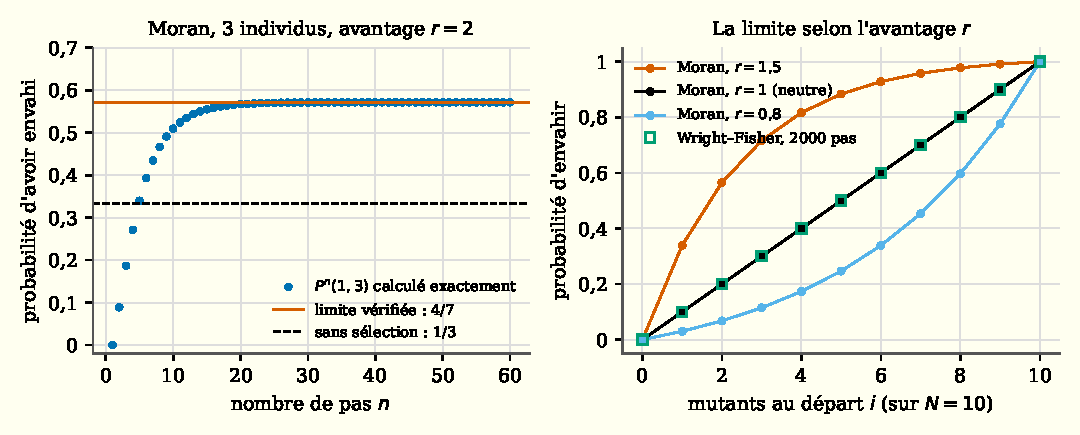
\includegraphics[width=\linewidth]{figures/c06_fixation}
\caption{Probabilité d'avoir envahi après $n$ coups (gauche)~; chance finale selon l'avantage $r$ (droite).}
\label{fig:c06}
\end{figure}

\section*{Comment on s'est assuré que ce n'est pas faux}

En résumé~: \niveau{A} pour les énoncés sur les puissances de matrices, \niveau{C} pour leur lecture en termes de
trajectoires, \niveau{X} pour la simulation.

Pour les énoncés démontrés, \og le juge a regardé\fg~: le noyau Lean a vérifié chaque étape,
et les seules hypothèses de départ admises (les \og axiomes\fg) restent dans une courte liste blanche de trois
principes standard. Un agent d'IA distinct de celui qui a produit le travail, mais de la même famille de modèles, a
tout reconstruit depuis les sources dans son propre répertoire~: les 14 énoncés de niveau A
repassent. Il a aussi planté des pièges, qui devaient échouer et ont échoué~:
\begin{itemize}
\item une \og preuve\fg{} d'une fausse limite, bouchée par un trou (\texttt{sorry}) ou par un axiome inventé~: le
  fichier se compile quand même sans erreur, mais l'audit des axiomes signale la tricherie~;
\item la valeur vérifiée $4/7$ remplacée par $1/3$~: le noyau refuse.
\end{itemize}
Une contre-épreuve figure dans les théorèmes eux-mêmes~: une chaîne qui a bien ses deux bouts pièges et une
fonction d'arrivée cohérente, mais qui n'est jamais absorbée. Elle montre que la condition de variance n'est pas
décorative. L'auditeur a refait le calcul numérique et obtenu un fichier identique octet pour octet, et le rejeu
complet des démonstrations dans le noyau, le 26 octobre 2026, est passé sans erreur. Le
registre des revendications reste pourtant à \og non audité\fg~: aucun humain n'a encore relu que les énoncés Lean
disent bien ce que leurs résumés en français annoncent.

\section*{Ce que ça ne dit pas}

\begin{limite}
\begin{itemize}
\item Rien de neuf en biologie~: ce sont des résultats de manuel, et le travail ne revendique aucune priorité. La
  nouveauté est qu'un vérificateur les a contrôlés, et que les briques sont réutilisables.
\item Le noyau a vérifié des limites de puissances de matrices. Qu'elles soient \og la probabilité d'atteindre $N$
  avant le temps $n$\fg{} est la définition standard, mais ce lien n'est pas formalisé (\niveau{C}).
\item Un objectif annoncé à l'avance, le théorème fondamental de Fisher sous sa forme générale, \emph{n'a pas été
  atteint}~; seul un cas particulier simple est démontré.
\item Les calculs CVODE sont une esquisse \niveau{X}~: ils illustrent, ils ne prouvent rien.
\item Les articles originaux de 1958, 1970 et 1972 n'ont pas été lus directement, ce que l'article dit lui-même.
\end{itemize}
\end{limite}

\section*{Pour aller plus loin}

L'article, son registre et l'audit sont déposés sous doi:10.5281/\allowbreak zenodo.23653850. Les briques \og absorption\fg{}
et \og modèle de Moran\fg{} sont réutilisées telles quelles par le travail sur le théorème isotherme, qui passe de la
population bien mélangée à la population posée sur un réseau (doi:10.5281/zenodo.23660071).
